\documentclass[preview,border=2pt]{standalone}
\usepackage{pgfplots}
\pgfplotsset{compat=1.18}

\begin{document}

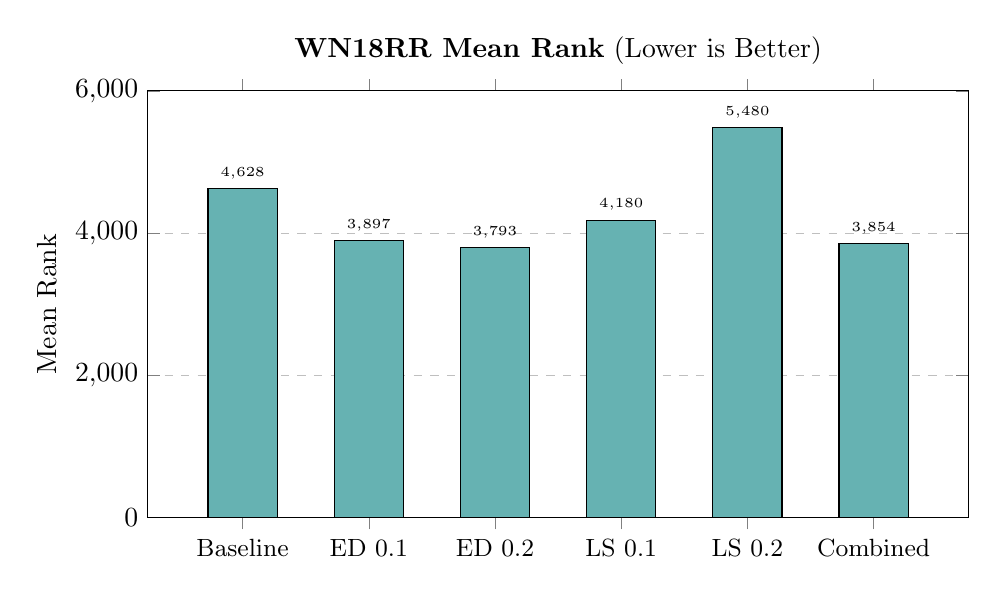
\begin{tikzpicture}
    \begin{axis}[
        ybar,
        title={\textbf{WN18RR Mean Rank} (Lower is Better)},
        width=12cm,
        height=7cm,
        symbolic x coords={Baseline, ED 0.1, ED 0.2, LS 0.1, LS 0.2, Combined},
        xtick=data,
        nodes near coords,
        nodes near coords style={font=\tiny, anchor=south},
        ymin=0, ymax=6000,
        ylabel={Mean Rank},
        ymajorgrids=true,
        grid style=dashed,
        bar width=25pt,
        enlarge x limits=0.15,
        xticklabel style={rotate=0, font=\small},
    ]
    
    % Data for WN18RR
    % Values: Baseline: 4628, ED 0.1: 3897, ED 0.2: 3793, LS 0.1: 4180, LS 0.2: 5480, Combined: 3854
    \addplot[fill=teal!60!white, draw=black] coordinates {
        (Baseline, 4628)
        (ED 0.1, 3897)
        (ED 0.2, 3793)
        (LS 0.1, 4180)
        (LS 0.2, 5480)
        (Combined, 3854)
    };
    \end{axis}
\end{tikzpicture}

\vspace{1cm}

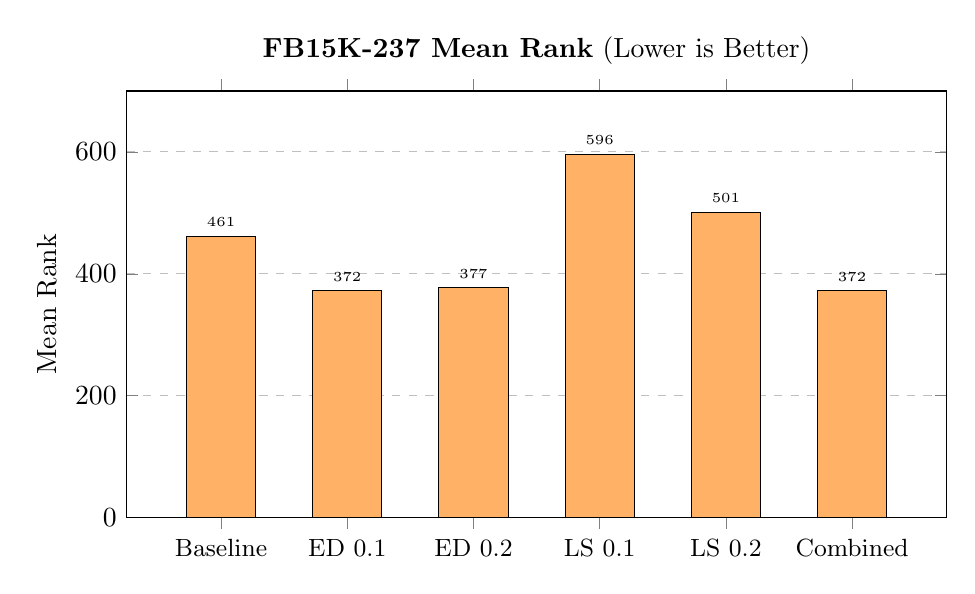
\begin{tikzpicture}
    \begin{axis}[
        ybar,
        title={\textbf{FB15K-237 Mean Rank} (Lower is Better)},
        width=12cm,
        height=7cm,
        symbolic x coords={Baseline, ED 0.1, ED 0.2, LS 0.1, LS 0.2, Combined},
        xtick=data,
        nodes near coords,
        nodes near coords style={font=\tiny, anchor=south},
        ymin=0, ymax=700,
        ylabel={Mean Rank},
        ymajorgrids=true,
        grid style=dashed,
        bar width=25pt,
        enlarge x limits=0.15,
        xticklabel style={rotate=0, font=\small},
    ]
    
    % Data for FB15K-237
    % Values: Baseline: 461, ED 0.1: 372, ED 0.2: 377, LS 0.1: 596, LS 0.2: 501, Combined: 372
    \addplot[fill=orange!60!white, draw=black] coordinates {
        (Baseline, 461)
        (ED 0.1, 372)
        (ED 0.2, 377)
        (LS 0.1, 596)
        (LS 0.2, 501)
        (Combined, 372)
    };
    \end{axis}
\end{tikzpicture}

\end{document}